\documentclass{article}
\usepackage[utf8]{inputenc}
\usepackage[english]{babel}
\usepackage{amsthm, amssymb, amsmath, amsfonts, extramarks}
\usepackage{gen, color}
\usepackage{graphicx}

\title{\vspace{-2cm}Homework Assignment 6}

\author{Bailey Wickham \& Alex MacLean\\ CSC530}

\date\today

\newenvironment{homeworkProblem}[1]{
    \section*{Problem #1}
}

\newenvironment{solution}{\color{blue} \em }{}



\setlength\textwidth{6.5in}
\setlength\textheight{8.75in}
\setlength\oddsidemargin{0in}
\setlength\evensidemargin{1in}
\setlength\topmargin{-0.25in}
\setlength\parindent{0in}
\setlength\parskip{0.5em}

\begin{document}
\maketitle

\section{Propositional Logic and Normal Forms}


\begin{enumerate}
\item (5 points) \label{prob:classify} Use the solution skeleton in \texttt{classify.rkt},
write a Rosette procedure that takes as input a formula $F$ in propositional logic and outputs
\begin{itemize}
	\item \texttt{'TAUTOLOGY} if $I \models F$ for every interpretation $I$;
	\item \texttt{'CONTRADICTION} if $I \not\models F$ for every interpretation $I$; and,
	\item \texttt{'CONTINGENCY} if there are two interpretations $I$ and $I'$ such that $I\models F$ and $I'\not\models F$.
\end{itemize}
Your procedure may contain at most two solver-aided queries (such as \texttt{solve}),
	and if it contains more than one query, then the two queries must be different (i.e., you cannot use \texttt{solve} twice).

\begin{solution}
	See \texttt{classify.rkt}
\end{solution}

\item (5 points)  Convert the following formula to an equisatisfiable one in CNF using Tseitin's encoding:
\[\neg ( \neg r \rightarrow \neg (p \land q))\]
Write the final CNF as the answer.
Use $a_\phi$ to denote the auxiliary variable for the formula $\phi$;
for example, $a_{p\wedge q}$ should be used to denote the auxiliary variable for $p\wedge q$.
Your conversion should not introduce auxiliary variables for negations.

\begin{solution}

\[
\begin{array}{ll}
a_{\phi} & \land \\
( a_{\phi} \leftrightarrow \neg (\neg r \rightarrow \neg a_{p \wedge q})) & \land \\
(a_{p\wedge q} \leftrightarrow (p \wedge q)) &  \\
\end{array}
\]
\begin{align*}
    (a_{\phi} \leftrightarrow \neg (\neg r \rightarrow \neg a_{p \wedge q})) &\equiv
(\neg a_\phi \lor \neg r) \land (\neg a_\phi \lor a_{p \land q}) \land (r \lor \neg a_{p \land q} \lor a_\phi) \\
    (a_{p\wedge q} \leftrightarrow (p \wedge q)) &\equiv
    (\neg a_{p\wedge q} \lor p ) \land (\neg a_{p\land q} \lor q) \wedge (\neg p \lor \neg q \lor a_{p\wedge q})
\end{align*}
\[
a_\phi \land
(\neg a_\phi \lor \neg r) \land (\neg a_\phi \lor a_{p \land q}) \land (r \lor \neg a_{p \land q} \lor a_\phi) \land
(\neg a_{p\wedge q} \lor p ) \land (\neg a_{p\land q} \lor q) \wedge (\neg p \lor \neg q \lor a_{p\wedge q})
\]

\end{solution}

\item (10 points)  Let $\phi$ be a propositional formula in NNF, and let $I$ be an interpretation of $\phi$. Let the \emph{positive set} of $I$ with respect to $\phi$, denoted $\emph{pos}(I, \phi)$, be the literals of $\phi$ that are satisfied by $I$. As an example, for the NNF formula $\phi = (\neg r \land p) \lor q$ and the interpretation $I = [r \mapsto \bot, p \mapsto \top, q \mapsto \bot]$, we have $\emph{pos}(I, \phi) = \{ \neg r, p \}$. Prove the following theorem about the monotonicity of NNF:

{\bf Monotonicity of NNF:} For every interpretation $I$ and $I'$ such that $\emph{pos}(I, \phi) \subseteq \emph{pos}(I', \phi)$, if $I \models \phi$, then $I' \models \phi$.

(\textbf{Hint:} Use structural induction.) \label{prob:NNF}

\begin{solution}
\begin{proof}
    Proceed by structural induction.

\item \textbf{Base case:} Suppose that $\phi$ is a literal of the form $p$ or $\neg p$ and $I$ is an interpretation such that $I \models \phi$. Then $pos(I, \phi)$ must contain $p$ or $\neg p$ respectively. Since $\emph{pos}(I, \phi) \subseteq \emph{pos}(I', \phi)$ then that element must also be in $\emph{pos}(I', \phi)$. Therefore $I' \models \phi$.

\item \textbf{Inductive hypothesis:} Suppose there exists a $\phi_1$ and $\phi_2$ such that for every interpretation $I$ and $I'$ such that $\emph{pos}(I, \phi_i) \subseteq \emph{pos}(I', \phi_i)$, if $I \models \phi_i$, then $I' \models \phi_i$.

\item \textbf{Inductive step:}
    Let $\phi = \phi_1 \land \phi_2$ and $I$ be an interpretation such that $I \models \phi$. Because $I \models \phi$ by the semantics of propositional logic $I \models \phi_1$. Since $\phi$ contains all the literals in $\phi_1$ then $pos(I, \phi_1) \subseteq pos(I, \phi)$. For any interpretation $I'$ such that $pos(I, \phi) \subseteq pos(I', \phi)$ then $pos(I, \phi_1) \subseteq pos(I', \phi_1)$.  Since $I \models \phi_1$ and $pos(I, \phi_1) \subseteq pos(I', \phi_1)$ by the inductive hypothesis $I' \models \phi_1$. A similar argument can be applied to $\phi_2$. Since $I' \models \phi_1$ and $I' \models \phi_2$, $I' \models \phi$.
The case for $\phi = \phi_1 \lor \phi_2$ follows similarly.

\item \textbf{Conclusion:} By induction, every interpretation $I$ and $I'$ such that $\emph{pos}(I, \phi) \subseteq \emph{pos}(I', \phi)$, if $I \models \phi$, then $I' \models \phi$.
\end{proof}
\end{solution}


\item (10 points) Let $\phi$ be an NNF formula.  Let $\hat{\phi}$ be a formula derived from $\phi$ using a modified version of Tseitin's encoding in which the CNF constraints are derived from implications rather than bi-implications.   For example, given the formula
\[a_1\land (a_2 \lor \neg a_3),\]
the new encoding is the CNF equivalent of the following, where $x_0, x_1, x_2$ are fresh auxiliary variables:\looseness=-1
\[
\begin{array}{ll}
x_0 & \land \\
(x_0 \rightarrow a_1 \land x_1) & \land \\
(x_1 \rightarrow a_2 \lor x_2) & \land \\
(x_2 \rightarrow \neg a_3) &  \\
\end{array}
\]
Note that Tseitin's encoding to CNF starts with the same formula, except that $\rightarrow$ is replaced with $\leftrightarrow$.  As a result, the new encoding has roughly half as many clauses as the Tseitin's encoding.

\medskip
Prove that $\hat{\phi}$ is satisfiable if and only if $\phi$ is satisfiable.

\medskip
(\textbf{Hint}: Use the theorem from Problem \ref{prob:NNF}.)

\begin{solution}
	\begin{proof}
		If there exists an interpretation $I$, such that $I \models \phi$, then an interpretation $I'$ such that $I' \models \hat{\phi}$ can always be constructed from it. This can be accomplished by setting the literals in $I'$ to there values in $I$ and setting the fresh auxiliary variables generated by the algorithm to the truth values the clauses they represent in $I \models \phi$. This works because the clauses that the auxiliary variables are being substituted into will evaluate to the same truth values as they do in $\phi$ and the implication clauses added to the CNF will all be true because $\top \rightarrow \top \equiv \top$ and $\bot \rightarrow \bot \equiv \top$.
		
		\item The reverse is also true, if there exists an interpretation $I$, such that $I \models \hat{\phi}$, then an interpretation $I'$ such that $I' \models \phi$ can always be constructed from it. This can be accomplished by simply removing the auxiliary variables from $I$. This new interpretation will always satisfy $\phi$ because if the truth value of the clause is the same as the one assigned to the auxiliary variable then substituting it in will not change anything. Since the auxiliary variable implies the clause it is substituted for the only other possibility is that the auxiliary variable is $\bot$ while the cause evaluates to $\top$. Since the auxiliary variables will only occur in conjunctions and disjunctions substituting $\bot$ for $\top$ in an expression that evaluates to $\top$ cannot possibly cause it to evaluate to $\bot$.
		
		\item Therefore if $\phi$ is satisfiable then $\hat{\phi}$ is also satisfiable and vice versa so $\hat{\phi}$ is satisfiable if and only if $\phi$ is satisfiable.
	\end{proof}
\end{solution}

\end{enumerate}

\pagebreak

\section{SAT solving (20 points)}\label{solving}


\begin{enumerate}
	\setcounter{enumi}{4}

	\item (20 points) In this problem, you will trace the execution of CaDiCaL, a high-performance SAT solver, on a sample CNF, and use this trace to reconstruct the abstract state transitions of the underlying CDCL algorithm (Lecture 4).

	The sample CNF is given in the DIMACS format and represents the following clauses:
	\begin{center}
		$(\neg x_1 \lor x_2 \lor x_4) \wedge (x_1 \lor x_3)  \wedge (\neg x_4 \lor \neg x_2) \wedge (\neg x_4 \lor \neg x_1 \lor x_2)  \wedge (x_3 \lor \neg x_1)  \wedge (\neg x_3 \lor \neg x_2 \lor x_4) \wedge (x_1 \lor x_4) \wedge (\neg x_2 \lor x_1)$
	\end{center}

	To start, clone CaDiCaL from GitHub and checkout tag \texttt{sc18}. Next, follow the instructions in the included \texttt{README.md} file to configure and build the solver in logging mode using \texttt{./configure -l \&\& make}. Finally, run the solver (in \texttt{build/cadical}) with the logging (\texttt{-l}) option on \texttt{sample.cnf}, and the solver will output a detailed trace of its execution.

	Using this detailed trace, reconstruct the behavior of the underlying CDCL algorithm by filling out the following abstract trace template, given as a list of abstract trace entries:

	\begin{itemize}
		\item \textbf{Level} \textcolor{DarkGreen}{$i$}  \hfill{\textcolor{DarkGreen}{\emph{; decision level $i$}}}
		\begin{itemize}
			\item \textbf{Decision:} \textcolor{DarkGreen}{$d_i$}  \hfill{\textcolor{DarkGreen}{\emph{; decision literal at level $i$ or NA if level due to backtracking}}}
			\item \textbf{BCP:} \textcolor{DarkGreen}{$p_{i_0}, \ldots, p_{i_n}$} \hfill{\textcolor{DarkGreen}{\emph{; literals inferred by BCP at level $i$, in the detailed trace order}}}
			\item \textbf{Conflict Clause:}  \textcolor{DarkGreen}{$l_{i_0} \ldots l_{i_k}$} \hfill{\textcolor{DarkGreen}{\emph{; conflict clause or NA if no conflict at level $i$}}}

			\item \textbf{Implication Graph:} \textcolor{DarkGreen}{graph image} \hfill{\textcolor{DarkGreen}{\emph{; implication graph at level $i$, visualized with GraphViz}}}

		\end{itemize}
		\item $\ldots$
	\end{itemize}

	To produce the abstract trace, create an abstract trace  entry (``Level'') whenever the decision level changes in the detailed trace due to a new decision or backtracking. When filling out the entry template, use the literal names from the detailed trace. For example, the solver will represent the literal $\neg x_1$ as \texttt{-1}. Use GraphViz to visualize the implication graph at a given level. The \texttt{impl-graph.dot} file shows an example of how to specify implication graphs with GraphViz. Use the LaTeX \texttt{\textbackslash includegraphics} command to insert the resulting graph images into your \texttt{hw1.pdf} file.


\begin{solution}
	\begin{itemize}
\item \textbf{Level} 1
\begin{itemize}
	\item \textbf{Decision:} 1
	\item \textbf{BCP:} 3
	\item \textbf{Conflict Clause:} NA
	\item \textbf{Implication Graph:} 
	\begin{figure}[h!]
		\begin{center}
			
\includegraphics[scale=0.75]{sat-images/graph1}
		\end{center}
	\end{figure}
\end{itemize}

\pagebreak

\item \textbf{Level} 2
\begin{itemize}
	\item \textbf{Decision:} 2
	\item \textbf{BCP:} -4
	\item \textbf{Conflict Clause:} 4 -2 -3 learned -3 -2
	\item \textbf{Implication Graph:}
	\begin{figure}[h!]
		\begin{center}
			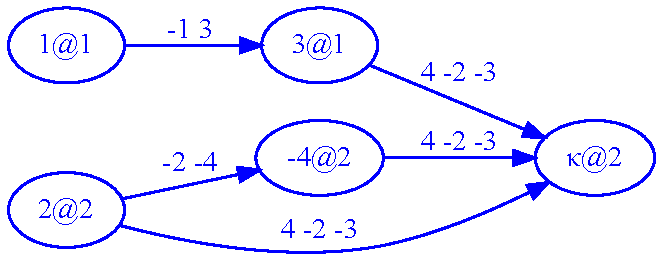
\includegraphics[scale=0.75]{sat-images/graph2}
		\end{center}
	\end{figure}
\end{itemize}

\item \textbf{Level} 1
\begin{itemize}
	\item \textbf{Decision:} NA
	\item \textbf{BCP:} -2, 4
	\item \textbf{Conflict Clause:} -4 2 -1 learned -1
	\item \textbf{Implication Graph:}
	\begin{figure}[h!]
		\begin{center}
			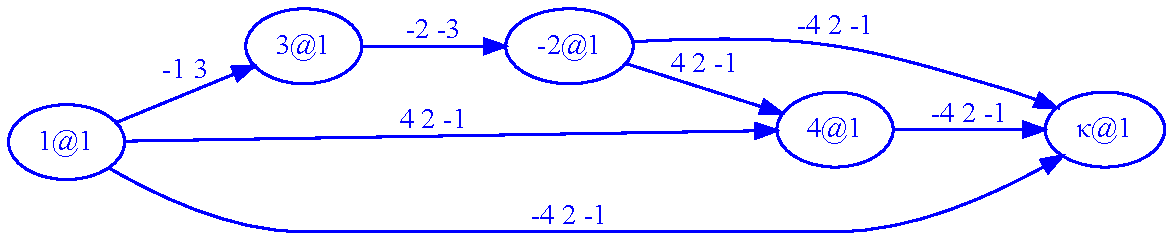
\includegraphics[scale=0.75]{sat-images/graph3}
		\end{center}
	\end{figure}
\end{itemize}

\item \textbf{Level} 0
\begin{itemize}
	\item \textbf{Decision:} NA
	\item \textbf{BCP:} -1, 3, 4, -2
	\item \textbf{Conflict Clause:} NA
	\item \textbf{Implication Graph:} 
	\begin{figure}[h!]
		\begin{center}
			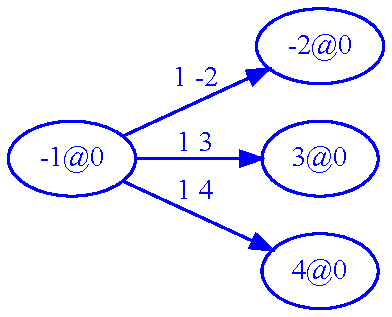
\includegraphics[scale=0.75]{sat-images/graph4}
		\end{center}
	\end{figure}
\end{itemize}
	\end{itemize}
\end{solution}

\end{enumerate}

\pagebreak

\section{Graph Coloring with SAT (40 points)}\label{coloring}

A graph is \emph{k-colorable} if there is an assignment of $k$ colors to its vertices such that no two adjacent vertices have the same color.  Deciding if such a coloring exists is a classic NP-complete problem with many practical applications, such as register allocation in compilers.  In this problem, you will develop a CNF encoding for graph coloring and apply them to graphs from various application domains, including course scheduling, N-queens puzzles, and register allocation for real code.

A finite graph $G = \langle V, E\rangle$ consists of vertices $V=\{v_1,\ldots,v_n\}$ and edges $E=\{\langle v_{i_1}, w_{i_1}\rangle,\ldots,\langle v_{i_m}, w_{i_m}\rangle\}$.  Given a set of $k$ colors $C=\{c_1,\ldots,c_k\}$, the \emph{k-coloring} problem for $G$ is to assign a color $c\in C$  to each vertex $v\in V$ such that for every edge $\langle v,w\rangle\in E$, $\mathsf{color}(v)\neq\mathsf{color}(w)$.

\begin{enumerate}
	\setcounter{enumi}{5}
\item (10 points) Show how to encode an instance of a $k$-coloring problem into a propositional formula $F$ that is satisfiable iff a $k$-coloring exists.
\begin{enumerate}
\item Describe a set of propositional constraints asserting that every vertex is colored.  Use the notation $\mathsf{color}(v) = c$ to indicate that a vertex $v$ has the color $c$.  Such an assertion is encodable as a single propositional variable $p^c_v$ (since the set of vertices and colors are both finite).

\begin{solution}
    $$\bigwedge_{v \in V} (\bigvee_{c \in C} p^c_v)  $$
\end{solution}

\item Describe a set of propositional constraints asserting that every vertex has at most one color.

\begin{solution}
    $$\bigwedge_{v \in V} \bigwedge_{c \in C} (p^c_v \rightarrow \neg (\bigvee_{c' \in C- \{c\}} p^{c'}_v))  $$
\end{solution}

\item Describe a set of propositional constraints asserting that no two adjacent vertices have the same color.

\begin{solution}
    $$\bigwedge_{\langle v, w \rangle \in E} \bigwedge_{c \in C} (\neg p_v^c \lor \neg p_w^c)  $$
\end{solution}

\item Identify a significant optimization in this encoding that reduces its size asymptotically.  (\textbf{Hint:} Can any constraints be dropped?  Why?)

\begin{solution}
    The constraint ensuring that each vertex has only 1 color (b) can be dropped.
    If the SAT solver assigns a vertex multiple colors this just means that any of them
    can be picked for a valid coloring.
\end{solution}

\item Specify your constraints in CNF.  For $|V|$ vertices, $|E|$ edges, and $k$ colors, how many variables and clauses does your encoding require?

\begin{solution}

$$
		P(G,C_k) = (\bigwedge_{\langle v, w \rangle \in E} \bigwedge_{c \in C} (\neg p_v^c \lor \neg p_w^c))
		          \land (\bigwedge_{v \in V} (\bigvee_{c \in C} p^c_v))
$$


     Clauses: $ k(|V| + |E|)$;
     Variables: $k|V|$

\end{solution}


\end{enumerate} \label{prob:encoding}

\item (20 points) \label{prob:kcol} Implement the above encoding in Racket, using the provided solution skeleton.  See the \texttt{README} file for instructions on obtaining solvers and the database of graph coloring problems.  Your program should generate the encoding for a given graph (see \texttt{graph.rkt}), call a SAT solver on it (\texttt{solver.rkt}), and then decode the result into an assignment of colors to vertices  (see \texttt{examples.rkt} and \texttt{k-coloring.rkt}).

Your implementation should be able to solve all of the easy and medium instances in under 15 minutes on an ordinary laptop.
(The reference implementation does so in about 7 minutes.)

\begin{solution}
	See \texttt{k-coloring.rkt}
\end{solution}

\item (5 points) Describe a CNF encoding for $k$-coloring that uses $O(|V|\log k+|E|\log k)$ variables and clauses.

\begin{solution}
    Instead of representing vertex coloring as $k$ literals, each literal corresponding to one possible color, Assign each color a number from $0$ to $k$, then use literals to represent the bits in a binary encoding of this number. This encoding will require $O(\log k)$ literals where $k$ is the number of colors. For each vertex a constraint will be required which translates
\end{solution}

\item (5 points) Most modern SAT solvers support \emph{incremental solving}---that is, obtaining a solution to a CNF, adding more constraints, obtaining another solution, and so on.  Because the solver keeps (some) learned clauses between invocations, incremental solving is  generally the fastest way to solve a series of related CNFs.  How would you apply incremental solving to your encoding from Problem \ref{prob:kcol} to find the smallest number of colors needed to color a graph (i.e., its chromatic number)?  \label{prob:last}

\begin{solution}

\end{solution}

\begin{solution}
    Start with the constraints generated by $P(G, C_{|V|})$, meaning each vertex has a unique color. We know that this is satisfiable. Next, add the constraint that none of vertices may be assigned the greatest color. Iteratively add this constraint until the problem is no longer satisfiable. Since we are only adding constraint, the SAT solver can use the previously calculated work to incrementally solve this problem. The coloring and the chromatic number correspond to the final satisfiable expression.
\end{solution}

\end{enumerate}


\section{Optimal Graph Coloring with Variations on SAT (10 points)}\label{varsat}


Consider the following variations on the propositional satisfiability (SAT) problem discussed in Lecture 5:

\begin{description}

	\item[Partial Weighted MaxSAT] Given a CNF formula $\phi_H = \bigwedge_{c \in H} c$ corresponding to a set of \emph{hard} clauses $H$, and a CNF formula $\phi_S = \bigwedge_{c \in S} c$ corresponding to a set of \emph{soft} CNF clauses $S$ with weights $w : S \rightarrow \mathbb{Z^+}$, the Partial Weighted MaxSAT problem is to find an assignment $A$ to the problem variables that satisfies all the hard clauses and that maximizes the weight of the satisfied soft clauses. That is, $A \models \bigwedge_{c \in H} c$, and if we let $C = \{ c\in S | A\models c\}$, then there is no $C'\subseteq S$ such that $H\cup C'$ is satisfiable and $\sum_{c'\in C'} w(c') > \sum_{c\in C} w(c)$.

	\item[Pseudo-Boolean Optimization]  Let $B$ be a set of \emph{pseudo-boolean constraints} of the form $\sum a_{ij}x_j \geq b_i$, where $x_j$ is a variable over $\{0, 1\}$ and $a_{ij}, b_i, c_j$ are integer constants.  The Pseudo-Boolean Optimization problem is to satisfy all constraints in $B$ while minimizing a linear function $\sum c_j \cdot x_j$.
\end{description}
%

Let $G = \langle V, E\rangle$ be a finite graph and $C_k = \{ c_1, \ldots, c_k \}$ a set of $k$ colors.
Let $P(G, C_k)$ be the CNF formula produced by applying your encoding from Problems \ref{prob:encoding}-\ref{prob:kcol}
to the graph $G$ and the coloring $C_k$.
As before, we use $p_v^c$ to denote the propositional variable indicating that the vertex $v\in V$ has the color $c\in C_k$.


\begin{enumerate}
	\setcounter{enumi}{9}

	\item (5 points) Explain how to create a Partial Weighted MaxSAT instance $P_{\text{opt}}(G)$
	such that every solution to $P_{\text{opt}}(G)$ represents a valid $\chi$-coloring of $G$ where $\chi$ is
	the chromatic number of $G$ (i.e., the smallest possible number of colors needed to color $G$).

	Your encoding of  $P_{\text{opt}}(G)$ may use $P(G, C_k)$ for at most one $k$ of your choosing.
	So, $P_{\text{opt}}(G)$ cannot use, for example, both $P(G, C_1)$ and $P(G, C_2)$.

	Write down  $P_{\text{opt}}(G)$ by specifying the set $H$ of hard clauses,
	the set $S$ of soft clauses, and the function $w : S \rightarrow \mathbb{Z^+}$ that assigns a positive weight to each soft clause in $S$.

\begin{solution}
	\begin{align*}
        H    	&=    P(G, C_{|V|}) \land \bigwedge_{c \in C_{|V|}} \bigwedge_{v \in V} (\neg p_v^c \lor \neg p_{unused}^c)  \\
        S    	&=     \bigwedge_{c \in C} p^c_{unused} \\
        w(s)    &=    1
	\end{align*}
\end{solution}

	\item (5 points)  Explain how to create a Pseudo-Boolean Optimization instance $P_{\text{opt}}(G)$
	such that every solution to $P_{\text{opt}}(G)$ represents a valid $\chi$-coloring of $G$ where $\chi$ is
	the chromatic number of $G$ (i.e., the smallest possible number of colors needed to color $G$).

	To create $P_{\text{opt}}(G)$, observe that every CNF instance
	can be transformed into a set of equivalent pseudo-boolean constraints.
	To apply this observation, explain how to do the transformation.

	As before, your encoding of  $P_{\text{opt}}(G)$ may use the  pseudo-boolean equivalent of  $P(G, C_k)$ for at most one $k$ of your choosing.


	Write down  $P_{\text{opt}}(G)$ by specifying the pseudo-boolean constraints to solve and the linear function to minimize:
    \begin{solution}
	\begin{align*}
        \text{minimize}  	 \quad& \sum_{c \in C} p^c_{used} \\
    \text{subject to } \quad& P(G, C_{|V|}) \land \bigwedge_{c \in C_{|V|}} \bigwedge_{v \in V} (\neg p_v^c \lor p_{used}^c)
	\end{align*}

	A CNF formula can be converted to a set of pseudo-boolean constraints by transforming each disjunctive sub-clause $C$ into a sum where $\sum_{c \in C} 1 \cdot c \geq 1$. The pseudo-booleans in this expression will all be of the from $p$ or $\neg p$. Every literal and it's negation must be related to each other by adding the following constraints as well.
	\begin{align*}
	(p) + (\neg p) &\geq 1 \quad&& \text{Ensures that either the predicate or the negation is true}\\
	-1 \cdot (p) + -1 \cdot (\neg p) &\geq -1 \quad&& \text{Ensures that either the predicate or the negation is false}
	\end{align*}
    \end{solution}

\end{enumerate}

\end{document}

